\documentclass[man, noapacite]{apa2}

\usepackage{hyperref}
% \usepackage{pslatex}
\usepackage{pdfsync}
\usepackage{apacite2}
\usepackage{amsmath}
\usepackage{graphicx}
\usepackage{topcapt}
\usepackage{color}

% don't split footnotes
\interfootnotelinepenalty=10000

% comment command
\newcommand{\blue}[1]{\textcolor{blue}{#1}}

\title{Negation is only hard to process when it is pragmatically uninformative}
% \title{Processing difficulty of negation is predicted by speakers' likelihood of using negation in context}
\author{Ann E. Nordmeyer and Michael C. Frank}
\affiliation{Department of Psychology, Stanford University}

\shorttitle{Pragmatics of negation}

\abstract{\blue{FIXME} Negation is a fundamental element of language and logical systems, but processing negative sentences can be challenging. Previous work suggests that a supportive context can mitigate the processing costs of negation.  We investigate the role of context on negative sentences by measuring the processing cost of negation in different contexts.  We find that a supportive visual context has a graded effect on negation processing.  Reaction times to respond to both positive and negative sentences were predicted by participants' descriptions of the same stimuli.  Our data suggest that in the right context, representing negation may be less difficult than previously supposed.}  

\acknowledgements{This material is based upon work supported by the National Science Foundation Graduate Research Fellowship. }

\begin{document}
\maketitle

%%%%%%%%% INTRO %%%%%%%%% 
\section{Introduction}

Language is a powerful tool that allows us to describe not only the state of the world as we see it, but also the world as it is not. Nevertheless, for human language users, processing negation is often slow and effortful. Deciding the truth value of a sentence like ``star isn't above plus'' takes a lot longer than making the same decision about a positive sentence \cite{hclark1972, carpenter1975, just1971, just1976}. And in language comprehension tasks, participants often show evidence consistent with having processed the positive components of a sentence prior to negating them, suggesting again that negation is challenging \cite{kaup2003, kaup2006, hasson2006, fischler1983, ludtke2008}. 

Yet not all negations are equally felicitous. For example, it would be strange to say ``my car isn't purple''---unless we are in a parking lot where every car except yours \emph{is} purple.  And it would be even weirder (though still true) to follow up by saying ``my car isn't a parakeet.''  On Gricean and neo-Gricean accounts of the pragmatics of language use in context, listeners expect speakers to produce informative and relevant utterances \cite{grice1975, horn1984, levinson2000, sperber1986}. The fact that your car is not purple is uninformative if it doesn't help me identify your car, and the subsequent remark about your car not being a parakeet is uninformative \emph{and} irrelevant.  Is this kind of pragmatic infelicity generally responsible for the processing cost of negation?

Consistent with this suggestion, presenting negative information in a supportive context can mitigate some of its processing costs \cite{wason1965, glenberg1999}. Contexts that explicitly mention a negated characteristic \cite{ludtke2006} or that present negation within a dialogue \cite{dale2011} tend especially to be processed faster.  And in an ERP experiment, contextually-supported negations (e.g., ``with proper equipment, scuba-diving isn't very dangerous'') elicited smaller N400 responses---a marker of semantic processing costs---than unlicensed negations \cite<e.g., ``bulletproof vests aren't very dangerous'';>{nieuwland2008}.

Although this previous work supports the idea that some kind of contextual expectations are the source of negation's processing cost, they do not specify the precise nature of these expectations. Drawing on a recent theoretical model of pragmatic reasoning \cite{frank2012}, we define pragmatic expectations in context as the probability that a speaker would utter a statement in order to convey a particular meaning. Our current experiment directly tests two hypotheses. First, expectations about what speakers would likely say---and their match or mismatch with what the speaker in fact \emph{does} say---are responsible for the processing costs of negation. Second, speakers tend to produce negated sentences only when they are both relevant and informative given the context.

In our experiment, we show participants sets of characters who are identical except for the presence or absence of a feature (e.g., boys with or without apples). In the \emph{speaker} condition, we ask participants to produce written descriptions that pick a particular target character out of the set, while in the \emph{listener} condition, we ask participants to evaluate the truth value of negative or positive statements about the target character. Our predictions are: A) that the processing cost for listeners of a negative sentence about a target picture should be predicted by how unlikely it is for a speaker to use negation to describe that target, and B) that speakers will produce sentences that effectively identify the referent of the sentence (i.e., that are informative) and that refer to a salient feature of the context (i.e., that are relevant).  

\section{Method}

\subsection{Participants} 

%NOTE: These ns are correct & checked
We recruited 489 participants (262 male and 224 female, three declined to report gender; ages 18 -- 65+) to participate in an online experiment through the Amazon's Mechanical Turk (mTurk) website.  We restricted participation to individuals in the US and paid 50 cents for this 10 minute study.  Participants were randomly assigned to either the speaker condition (n = 296) or the listener condition (n = 193).

\subsection{Stimuli}

\begin{figure}[t]
\begin{center} 
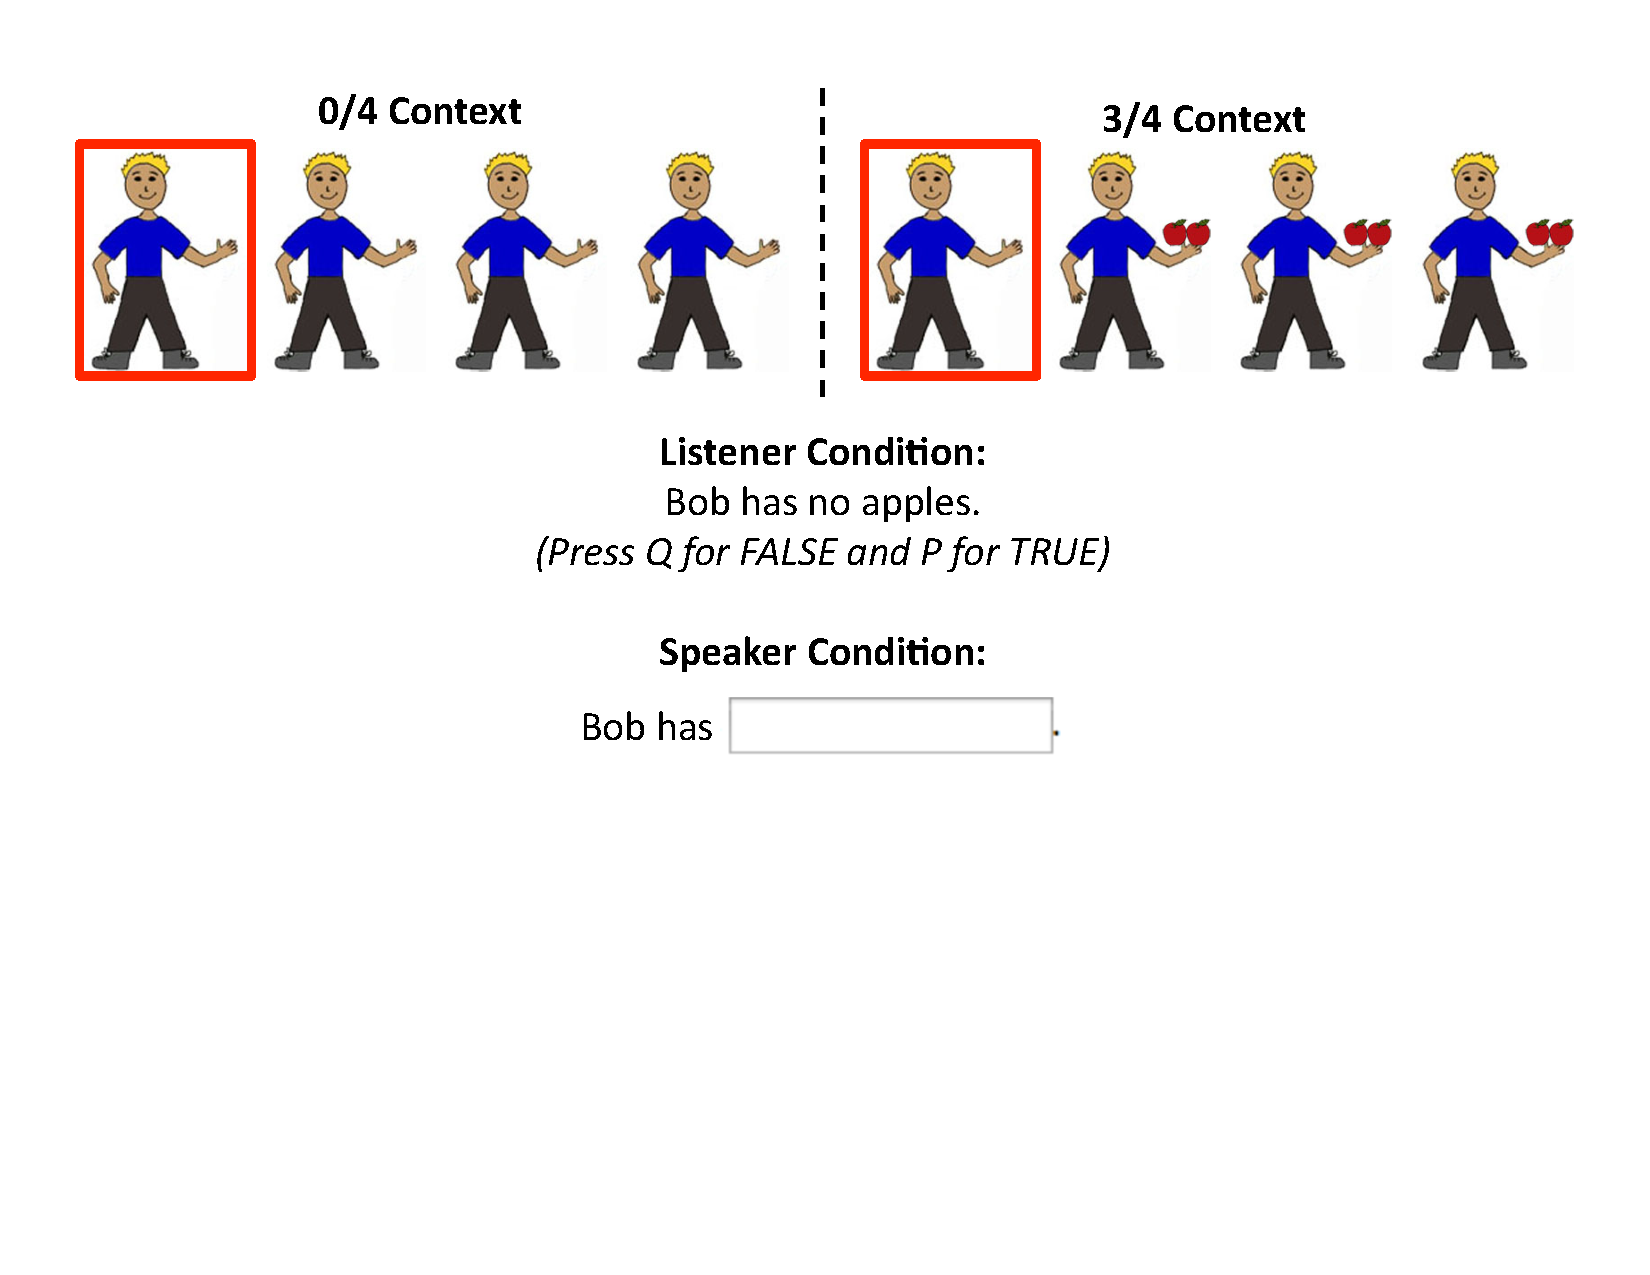
\includegraphics[width=4in]{figures/trialfig.pdf}
\caption{\label{fig:trial} An example of a true negative trial with a 3/4 context. \blue{Modify figure to show what text the two conditions saw, rather than putting in comment text?}}
\vspace{-5mm}
\end{center} 
\end{figure}

Thirty-two trial items were created in which characters were shown holding either two of the same common, recognizable objects (``target items'', e.g. two apples), or holding nothing.  Within each trial, all characters were identical except for the presence or absence of objects; characters varied in appearance (e.g. skin tone, hair color, clothing, gender) across trials.\footnote{Our previous work indicates that the results reported here are robust to a number of changes to the stimuli, including whether the context characters varied in appearance or not. Results from these previous experiments are reported in \citeA{nordmeyer2014}.} Each participant saw trials in which different proportions of characters were holding target items (context condition).  Context conditions showed $\frac{0}{4}$, $\frac{1}{4}$, $\frac{2}{4}$, $\frac{3}{4}$, or $\frac{4}{4}$ of the characters holding objects. The order of characters was shuffled on each trial, with the referent of the sentence appearing in a random position. 

For participants in the listener condition, on each trial a sentence of the form ``[NAME] [has/has no] [ITEM]'' appeared.  Half of the sentences were positive and half were negative, and they were paired with pictures such that half were true and half were false.  The experiment was fully crossed, with participants receiving eight true positive, eight false positive, eight true negative and eight false negative sentences distributed equally across context types in a randomized order over the course of the study.  \blue{How many trials per context? 8/5 is not a whole number.}

Participants in the speaker condition saw the same images paired with an incomplete sentence (e.g. ``[NAME] has $\rule{3cm}{0.15mm}$.''). In half of the trials, the highlighted picture was holding target items, and in half of the trials, the highlighted picture was holding nothing.  The experiment was fully crossed such that target characters appeared with or without target items an equal number of times in each context type.  

\subsection{Procedure}

Participants were first presented with a brief overview screen which explained that they would play a language game.  Once participants accepted the task, they were randomly assigned to either the listener condition or the speaker condition, and saw a more detailed instructions screen which explained the task and informed them that they could stop at any time.\footnote{The listener and speaker conditions of the experiment can be viewed at \url{https://langcog.stanford.edu/expts/AEN/negatronv20/negatron.html} and \url{https://langcog.stanford.edu/expts/AEN/negatron_production2/negatron.html}, respectively.}

In the listener condition, participants first saw eight positive sentence practice trials with feedback about incorrect responses before beginning the test trials. In each test trial, participants saw an array of four pictures presented in a random horizontal arrangement.  Participants were told to look at these pictures for four seconds, at which point a red box appeared around one of the pictures.  One second later, a sentence about that picture appeared.  Participants were told to read the sentence and respond as quickly and accurately as possible with a judgment of whether it was true or false when applied to the highlighted picture.  We recorded reaction times for each trial, measured as the time from when the sentence was presented to the moment when the response was made.

In the speaker condition, there were no practice trials. In each test trial, participants saw an array of four pictures: The target pictures and three context pictures presented in a random horizontal arrangement.  Participants were told to look at these pictures for four seconds, at which point a red box appeared around one of the pictures.  One second later, an incomplete sentence appeared.  Participants were told to finish the sentence (by typing into a small text box) using only a few words, in a way that would help someone else identify the character in the red box if they saw the pictures in a different order.
  
\subsection{Data Processing} 
  
We excluded 18 participants who did not list English as their native language and two participants from the listener condition for having an overall accuracy below 80\%, leaving a total of 469 participants for analysis (186 in listener condition, 283 in speaker condition). 

In the listener condition, we excluded trials with RTs greater than 3 standard deviations from the log-transformed mean, a criterion established in our previous experiments \cite{nordmeyer2014}.  Due to the Gricean motivation of our analysis, which led us to assume that speakers would be truthful as well as informative and relevant, we focused on predicting the processing of true or correct sentences.   

In the speaker condition, we coded participant's productions. Affirmative responses labeling the target feature were coded as ``positive'' (e.g., ``apples'', ``two apples'', ``red apples'', etc.).  Responses with a negative element (``no'', ``not'', ``nothing'', ``empty'', or ``zero'') were coded as ``negative.''  All other responses (e.g., descriptions of the characters' clothing or hair color) were coded as ``other.''  Codes were hand-checked to ensure that label synonyms or spelling errors were coded correctly.  

To predict responding in the listener condition, we used productions from the speaker condition. We calculated the proportion of positive sentences describing characters who possessed target items, and the proportion of negative sentences describing characters with nothing, creating a probability distribution for true positive and true negative utterances.  We then used this distribution to calculate the surprisal of hearing a positive or negative sentence for each trial type. Surprisal is an information-theoretic measure of the amount of information carried by an event; in prior work on sentence comprehension it has been used successfully as a linking hypothesis between production probabilities and reaction times \cite{levy2008}. Surprisal (or ``self-information'' $I$) for a sentence $s$ is defined as

\begin{equation}
\label{eq:surprise}
I(s) = -\log(P(s)).
\end{equation}

%NOTE: We should talk about the best way to present the speaker data.  What I've done here is pretty sparse (I really just jump right to surprisal, describing how we calculate that here and then describing the relationship between surprisal and RT in the results section.  I'm wondering if we should present a table of the probabilities in response to each trial type, though?)

\section{Results}

\subsection{Listener Condition}

\begin{figure}[t]
\begin{center} 
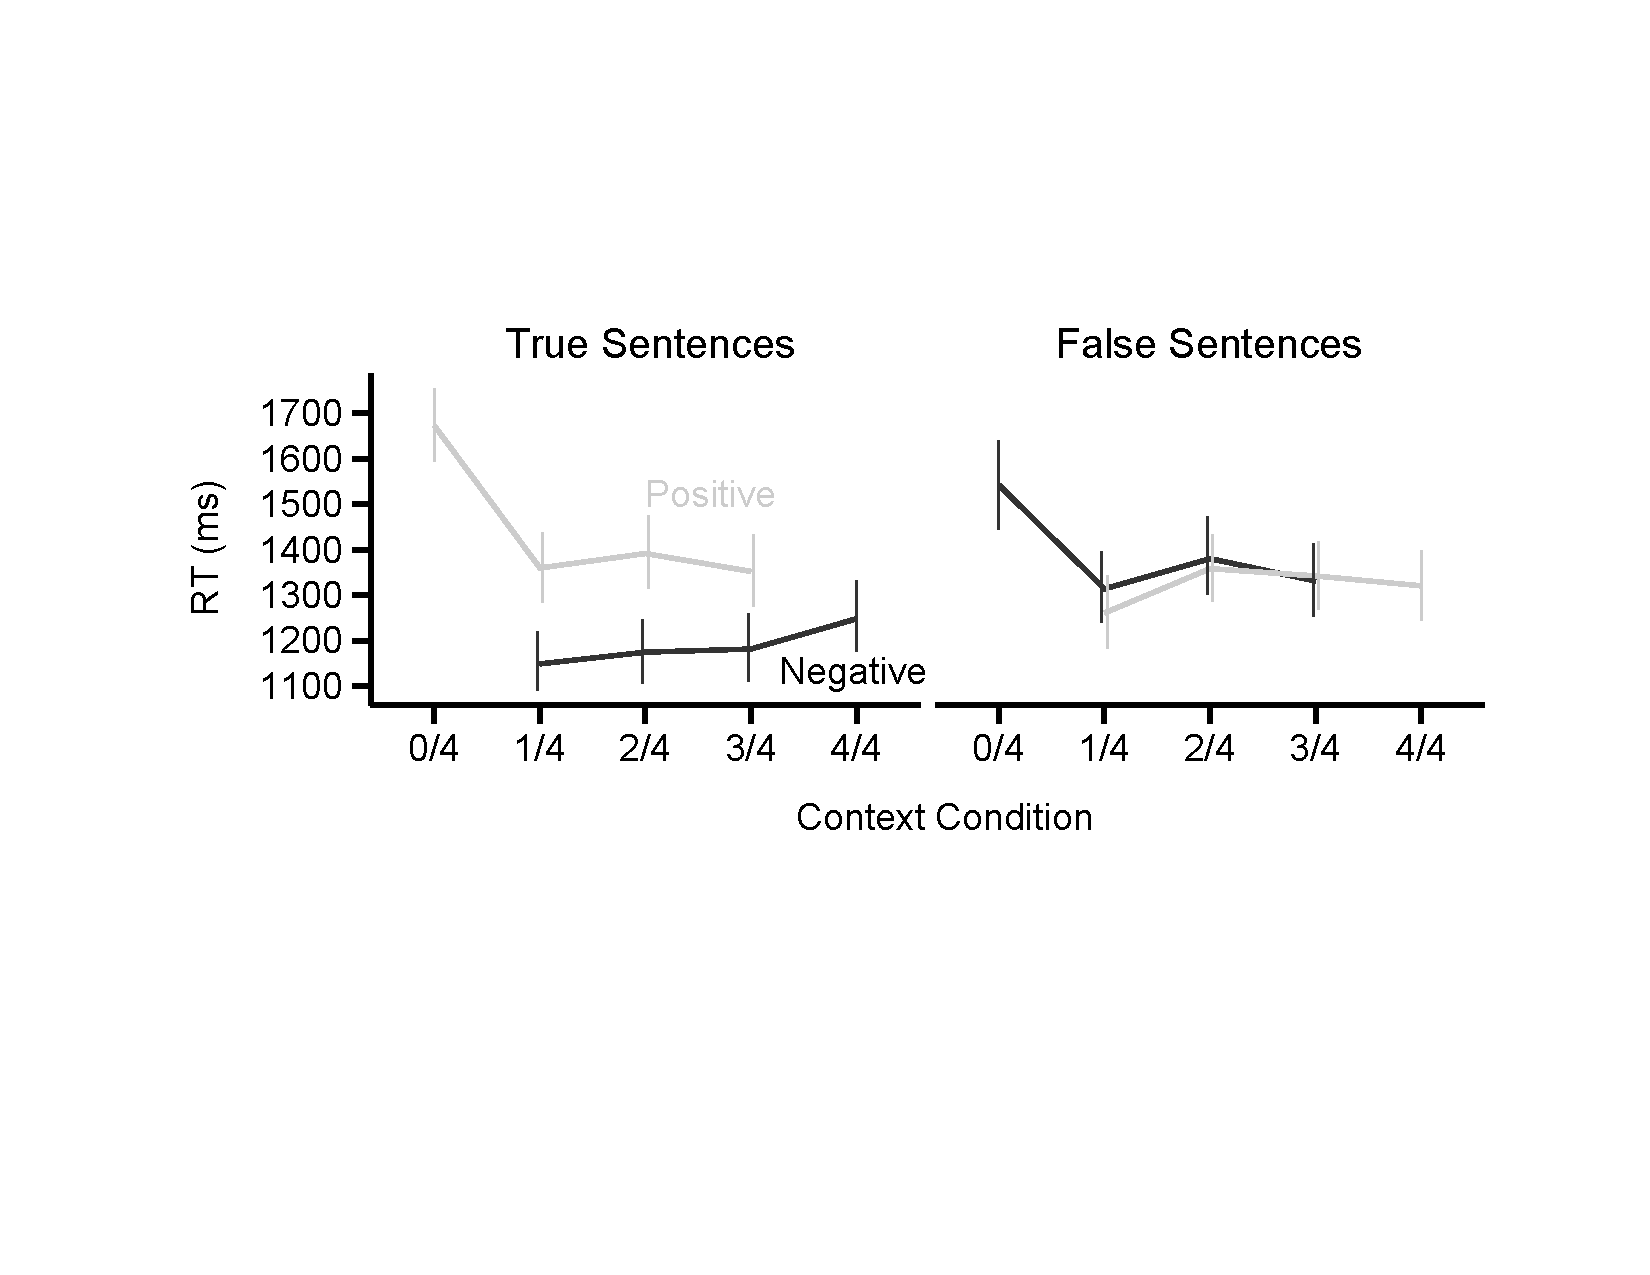
\includegraphics[width=4.5in]{figures/rts.pdf}
\caption{\label{fig:e2line} Reaction times for each trial type across different conditions. Responses to true sentences are shown on the left, and false sentences are shown on the right.  Negative sentences are shown in grey, and positive sentences in black.  The context condition is notated by a fraction representing the number of characters in the context who held target items. Error bars show 95\% confidence intervals computed by non-parametric bootstrap.}
\end{center} 
\end{figure}

Participants were fastest to respond to true positive sentences, and slowest to respond to true negative sentences, replicating previous findings \cite{hclark1972}.  Responses to true negative sentences showed the most pronounced effect of context, with reaction times in response to negative sentences decreasing as the proportion of target items in the context increased.  Responses to false positive sentences showed a similar but less pronounced effect of context, and responses to true positive and false negative sentences showed a slight but reversed effect of context, with increased reaction times as the proportion of target items in the context increased. \blue{This paragraph needs more intuition and less direct description.}

To evaluate the reliability of these patterns, we fit a linear mixed-effects model to reaction times in response to sentences.  We examined the interaction between sentence type (positive or negative), truth value (true or false), and context condition as predictors of reaction time. All mixed-effects models were fit using the lme4 package version 1.1-7 in R version 3.1.2.  The model specification was as follows: \texttt{RT $\sim$ sentence~$\times$~truth~$\times$~context + (sentence~\textbar~subject) +  (sentence~\textbar~item)}.  Significance was calculated using the standard normal approximation to the $t$ distribution \cite{barr2013}.\footnote{Raw data and analysis code can be found at \blue{FILL THIS IN LATER}.}

All model coefficients are shown in Table \ref{tab:model}. In addition to main effects of sentence type and truth value, the model showed an interaction these, such that true positive sentences elicited the fastest responses and true negative sentences elicited the slowest responses. The model showed a significant negative linear effect of context, with reaction times decreasing as the proportion of characters with target items increased. A significant three-way interaction between sentence type, truth value, and context indicates that this pattern was driven primarily by responses to true negative sentences, however, with true positive and false negative sentences showing a smaller positive linear effect of context.  

\begin{table}[t]
\caption{\label{tab:model} Coefficient estimates from a mixed-effects model predicting listeners' reaction times in response to sentences in different context conditions.}
\begin{center}
% \small\addtolength{\tabcolsep}{-5pt}
\begin{tabular}{rrrr}
  \hline
 & Coefficient & Std. err. & $t$ \\ 
  \hline
Intercept & 1541 & 45 & 34.20 \\ 
  Sentence (Negative) & -282 & 50 & -5.63  \\ 
  Truth (True) & -461 & 50 & -9.29 \\
  Context & -59 & 11 & -5.44 \\ 
  Sentence $\times$ Truth & 895 & 71 & 12.65 \\
  Sentence $\times$ Context & 78 & 15 & 5.05 \\
  Truth $\times$ Context & 92 & 15 & 5.97 \\
  Sentence $\times$ Truth $\times$ Context & -209 & 22 & -9.52 \\
   \hline
\end{tabular}
\vspace{-1.5cm}
\end{center}
\end{table}

\subsection{Speaker Condition}

\begin{figure}[t]
\begin{center} 
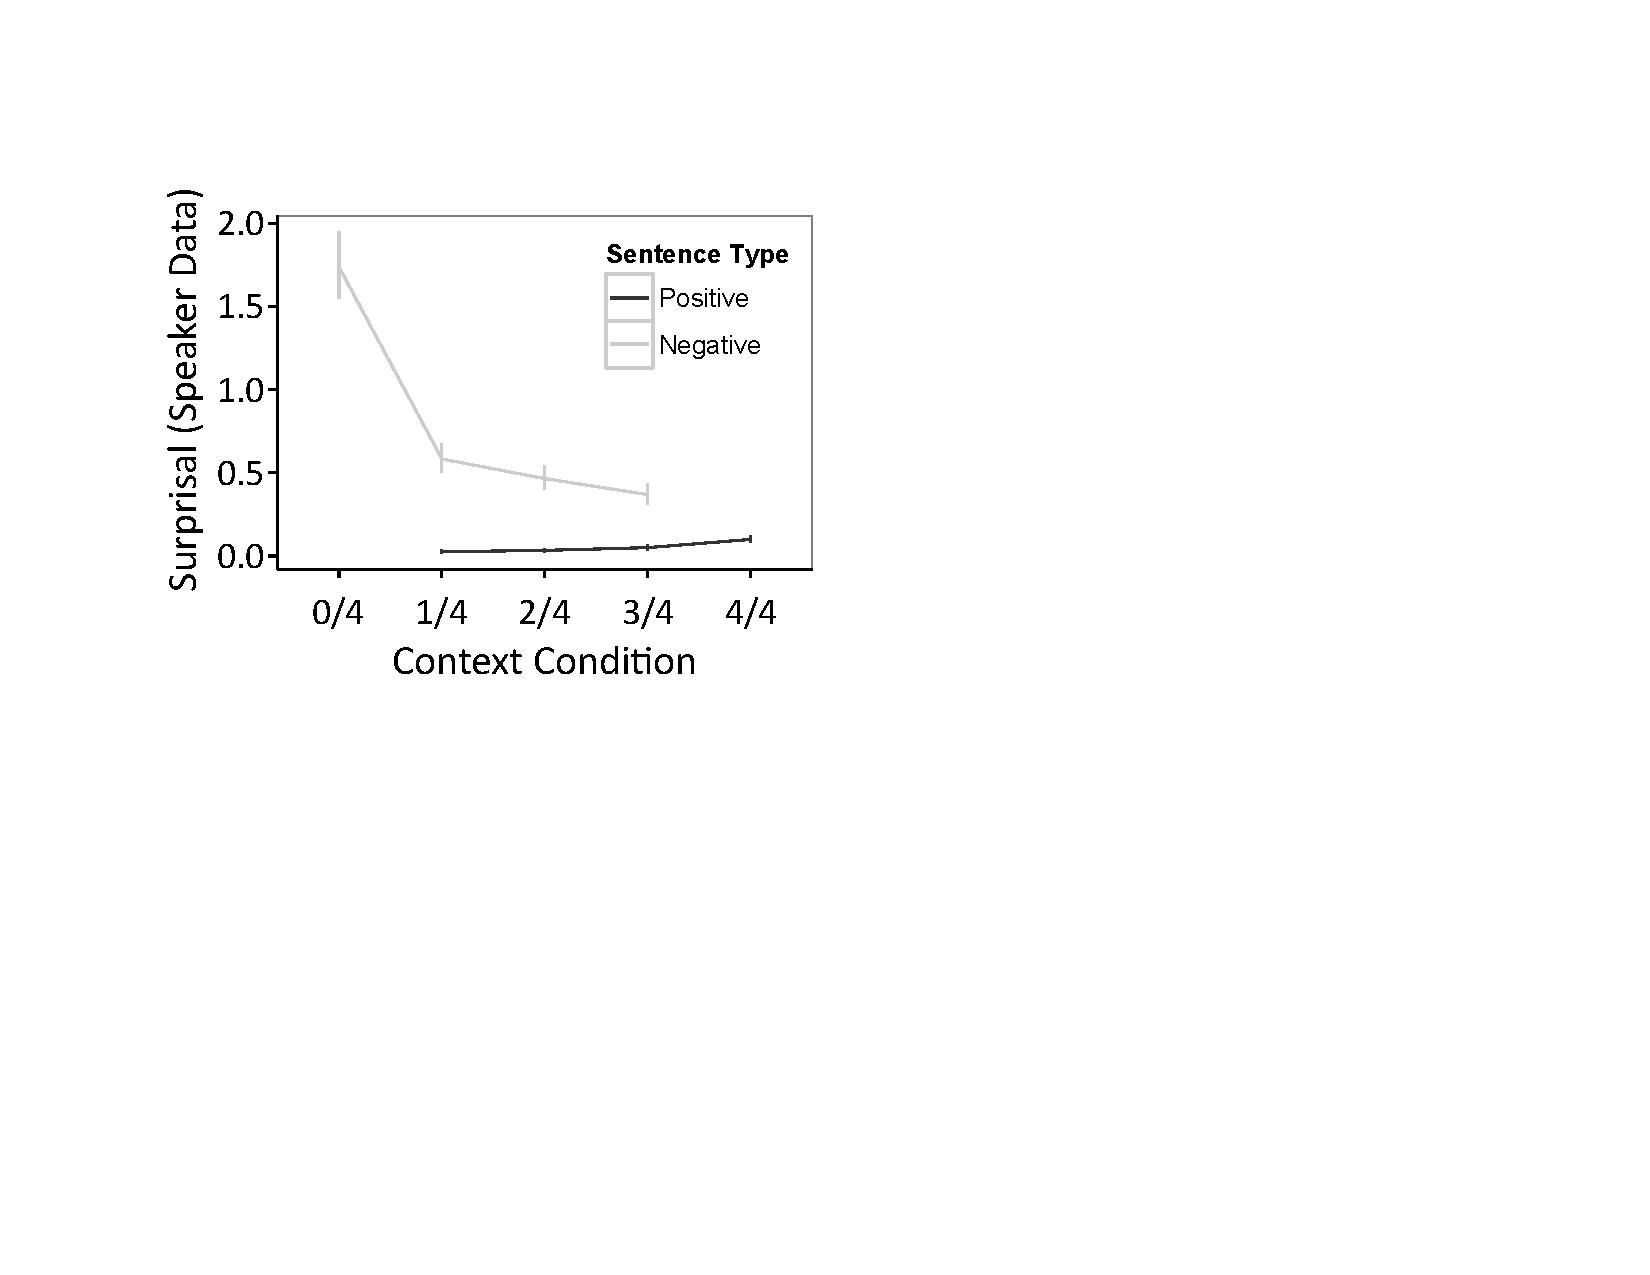
\includegraphics[width=3in]{figures/surprisals.pdf}
\caption{\label{fig:e2line} \textcolor{blue}{FIXME} Surprisal for true positive and true negative sentences across different conditions. On the left is a plot of surprisal computed using data from the speaker condition of the experiments.  Negative sentences are shown in grey, and positive sentences in black.  The context condition is notated by a fraction representing the number of characters in the context who held target items. Error bars show 95\% confidence intervals computed by non-parametric bootstrapping.  }
\end{center} 
\end{figure}

We hypothesized that the processing cost of negation could be explained by listeners' expectations about a speaker's potential utterance choices. In the speaker condition, surprisal was much higher for negative sentences compared to positive sentences across all context conditions.  Negative sentences in the $\frac{0}{4}$ condition had the highest surprisal, and positive sentences in the $\frac{1}{4}$ condition had the lowest surprisal.  For negative sentences, surprisal decreased as the number of characters with target items increased, and for positive sentences surprisal increased as the number of characters with target items increased.  \blue{Again, try to work in intuitions about WHY.}

% To link pragmatic expectations to reaction time, we assume that reaction time is proportional to \emph{surprisal}. Surprisal is an information-theoretic measure of the amount of information carried by an event (in this case, an utterance in some context) based on its probability. Surprisal has been used effectively to predict reaction times from probabilistic models \cite{levy2008}; here, we used the probability of participants in the speaker condition producing a true positive or a true negative utterance in different contexts to calculate pragmatic surprisal.

\begin{figure}[t]
\begin{center} 
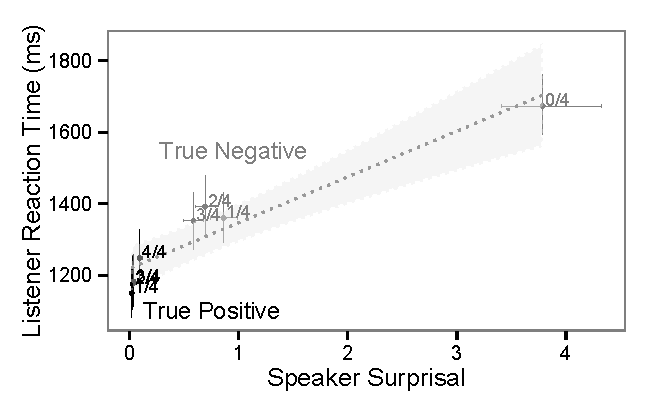
\includegraphics[width=4in]{figures/production_rts.pdf}
\caption{\label{fig:scatter} Reaction times in the listener condition plotted by surprisal in the speaker condition; each point represents a measurement for sentence type and context condition. Error bars on the horizontal and vertical axes represent 95\% confidence intervals on their respective measures.}
\end{center} 
\end{figure}

To test the hypothesis that processing times are a function of listeners' expectations about what a speaker will say, we regressed the mean reaction time in response to true positive and negative utterances in each condition against the surprisal for the same utterances (Figure \ref{fig:scatter}).  There was a significant positive relationship between surprisal and reaction time for true negative sentences, $r^2=.94$, $p<.001$, supporting our prediction that the effects of context on reaction time were driven by differences in how speakers would describe the same stimuli.  

\section{General Discussion}

What makes negation hard to process? While previous work has proposed that processing negative elements is especially difficult because of features intrinsic to negation, our work here suggests instead that this difficulty may not be unique to negation at all. Instead, general pragmatic mechanisms are likely responsible. Negative sentences presented without context are uninformative and irrelevant; thus, they are unlikely to be produced by speakers. In turn, comprehenders respond to these unlikely utterances with increased processing times. In contrast, in contexts where negation was more informative and relevant, processing costs are lower. Overall, this evidence supports a Gricean interpretation of the processing of negation.

While previous work has shown that contextual factors facilitate the processing of negation \cite{wason1965,nieuwland2008,dale2011}, our findings here go beyond these previous studies in a number of respects. First, and most importantly, by using actual language productions as the predictor of processing difficulty, our work strongly implicates specifically pragmatic (rather than semantic) factors. Second, rather than treating pragmatic as a black box, we show that two different components---informativeness and relevance---each contribute to the relative (un-)likelihood of heading a negation. Finally, by quantitatively manipulating the informativeness of particular descriptions in context, our experiment shows the graded nature of processors' expectations.

Our work here also uses surprisal, an information-theoretic measure of processing difficulty, as the linking hypothesis between speaker probabilities and reaction times \cite{levy2008}. Although this linking hypothesis has substantial support in the realm of syntactic processing \cite{demberg2008,boston2008}, to our knowledge, our findings are the first example of using surprisal over sentence-level pragmatic expectations, rather than word-level syntactic expectations. This success suggests that, in concert with the appropriate predictive models, surprisal theory could be productively applied to the prediction of processing difficulty beyond the level of syntax. 

Although our focus here was on negation, our findings has implications for sentence processing more generally.  Debates about the effects of pragmatics on linguistic processing exist in other domains, such as the processing of scalar implicatures \cite<the pragmatic inference that e.g., ``some'' implicates ``some but not all'';>{huang2009, huang2011, grodner2010}.  \citeA{tomlinson2013} provide an informative comparison between scalar implicature and negation, presenting mouse-tracking trajectories for each. Their negation data show the same pattern of processing difficulties we observe, and critically, their data on the processing of underinformative ``some'' utterances look almost identical. We hypothesize that, in both cases, participants' processing difficulty is a function of the violation of their pragmatic expectations.

Our findings here suggests that a large part of the processing difficulties in processing negation arise from the relative pragmatic felicity of negation in context. They do not rule out the possibility that there is some additional cost to processing an additional logical element, however, but this processing cost would have to be small with respect to the magnitude of the effects we observed. \blue{FINAL ASPIRATIONAL CONCLUSION?}

%  show the same mouse-tracking patterns in response to underinformative scalar implicatures as well as underinformative negative utterances.  

% We believe that formal models of pragmatics can provide insight into these debates and, more generally, into the role that pragmatic context plays in linguistic processing. 

% One contribution of our work here is that we use language production behavior to provide a strong operational definition of pragmatics.  Building on recent 

 % modeling work quantifies pragmatic reasoning based on the assumption that speakers are informative---they will produce utterances that pick out smaller subsets of the context, leaving as little ambiguity as possible for the listener \cite{frank2012,goodman2013}.  By this definition, negative sentences become more informative as the number of characters in the context increases.  This prediction is reflected in our results: Speakers were more likely to use negation in contexts where more people possessed the negated item.  

% We also found that both speakers' and listeners' behavior was strongly influenced by the presence of any target items in the context.  Speakers were much less likely to produce a negative utterance when none of the characters in the context possessed target objects; similarly, listeners took much longer to respond to these sentences than any of the other contexts.  We saw the same pattern in listeners' responses to false negative sentences.  These findings are consistent with relevance theory \cite{sperber1986}, as well as the idea that a speakers' utterances are influenced by the ``Question Under Discussion'' \cite{roberts1996}.  In addition to being uninformative, a sentence such as ``Bob has/has no apples'' in a context where none of the characters have apples is very strange, because ``apples'' is not a relevant feature of the context.  We interpret this finding as evidence for the role of relevance in producing and processing speech; in addition to being uninformative, these sentences might have incurred additional processing costs due to the mention of an unexpected topic.    

%Our analyses focused on true sentences, because of our interest in exploring participants' expectations about how an informative speaker should behave.  Due to the nature of our task, participants in the listener condition likely expected some of the sentences to be false, but it is not clear what constitutes an ``informative'' false sentence.  Our listener data replicate an interaction between sentence type and truth value that is seen frequently in literature on sentence verification tasks \cite{hclark1972}, with false positive sentences showing a similar pattern as true negative sentences.  




% These were contexts in which negation was informative (i.e., identified a narrower subset of the context) and relevant (i.e., the negated item was present in the context).  This pattern was also consistent with our Gricean hypothesis that the processing cost of negation is due to general pragmatic principles about how listeners expect speakers to behave.  

% In conversation, in contrast, negative sentences are often produced when some strong expectation has been violated, making the negation both informative and relevant. Congruent with that impression, 

% Our participants were faster to respond to negative sentences in contexts where speakers were more likely to use negation to describe the same stimuli. 

%We suggested a Gricean account of these data: The processing cost of negation is related to the degree to which it violates expectations about communication in context. In our studies, by changing the proportion of people in the context who held a target item, we systematically manipulated participants' contextual expectations.  We found a parametric relationship between the strength of the context and reaction times, and this relationship was well fit by participants' descriptions of the stimuli in different contexts.


 
 % and slower processing times.  


\bibliographystyle{apacite}

\setlength{\bibleftmargin}{.125in}
\setlength{\bibindent}{-\bibleftmargin}

\bibliography{negation}

\end{document}


%Maybe move some of this to the GD
%What is the mechanism by which context influences the processing of negation?  We propose that negative sentences are more informative in contexts that set up a strong expectation that is violated. If the processing cost of negation is pragmatic, then more informative negative sentences should elicit smaller reaction times. How should we quantify informativeness in context? Recent modeling work quantifies pragmatic reasoning in simple experimental contexts \cite{frank2012,goodman2013}. The assumption underlying this work is that speakers are informative---they will produce utterances that will pick out smaller subsets of the context, leaving as little ambiguity as possible for the listener.  We use this definition of informativeness to provide a quantitative interpretation of our hypothesis.

%MOVE THIS:
%To link pragmatic expectations to reaction time, we assume that reaction time is proportional to \emph{surprisal}. Surprisal is an information-theoretic measure of the amount of information carried by an event (in this case, an utterance in some context) based on its probability. Surprisal has been used effectively to predict reaction times from probabilistic models \cite{levy2008}; in this work, we directly measure the probability of an utterance occurring by eliciting descriptions of our stimuli from our participants.